\documentclass[11pt]{article}

%\usepackage{listings}
%\usepackage{float}
\usepackage{graphicx}
\usepackage{amsmath}
\usepackage{bm}
\usepackage{color}
%\usepackage{mathtools}

\newcommand\editremark[1]{{\color{red}#1}}

\title{Bayesian parameter inference on kilonova light curve data with \texttt{lc\_fit}}

\author{Elizabeth Champion}

\begin{document}

\maketitle

\section{Overview}

The \texttt{lc\_fit} code consists of independent \texttt{Python} scripts located in the \texttt{lc\_fit/bin/} directory. A parameter estimation run can be set up with the provided Makefile: for instance, running
\begin{verbatim}
	$ make test	
\end{verbatim}
sets up an injection-recovery test in the \texttt{lc\_fit/pe\_runs/} directory. Several things happen during this setup:
\begin{enumerate}
	\item An initial grid of samples is generated. This grid is sampled according to the prior distributions of the parameters. In particular, unless otherwise specified by the user, ejecta masses have log-uniform priors while the velocities and viewing angle have uniform priors.
	\item Two \texttt{HTCondor} DAG files are generated: one for generating the initial injection data, and one for performing the PE. \texttt{HTCondor} DAGs will be discussed futher below. For now, the important part is that they tell \texttt{HTCondor} what jobs to run and which of those jobs depend on other jobs completing first.
	\item A number of \texttt{HTCondor} submit files (ending with the extension \texttt{.sub}) are created. These files describe individual \texttt{HTCondor} jobs. In particular, they include the location of the executable (in our case \texttt{lc\_fit}'s \texttt{Python} code), the arguments to be supplied to the executable, and the location of any output or log files.
\end{enumerate}

Figure \ref{fig:flowchart} is a flowchart representing the algorithm at a high level. The usage instructions for each script in this flowchart are documented in the \texttt{lc\_fit} repository. The remainder of this document will describe the methods used in each stage of the algorithm.

\begin{figure}
	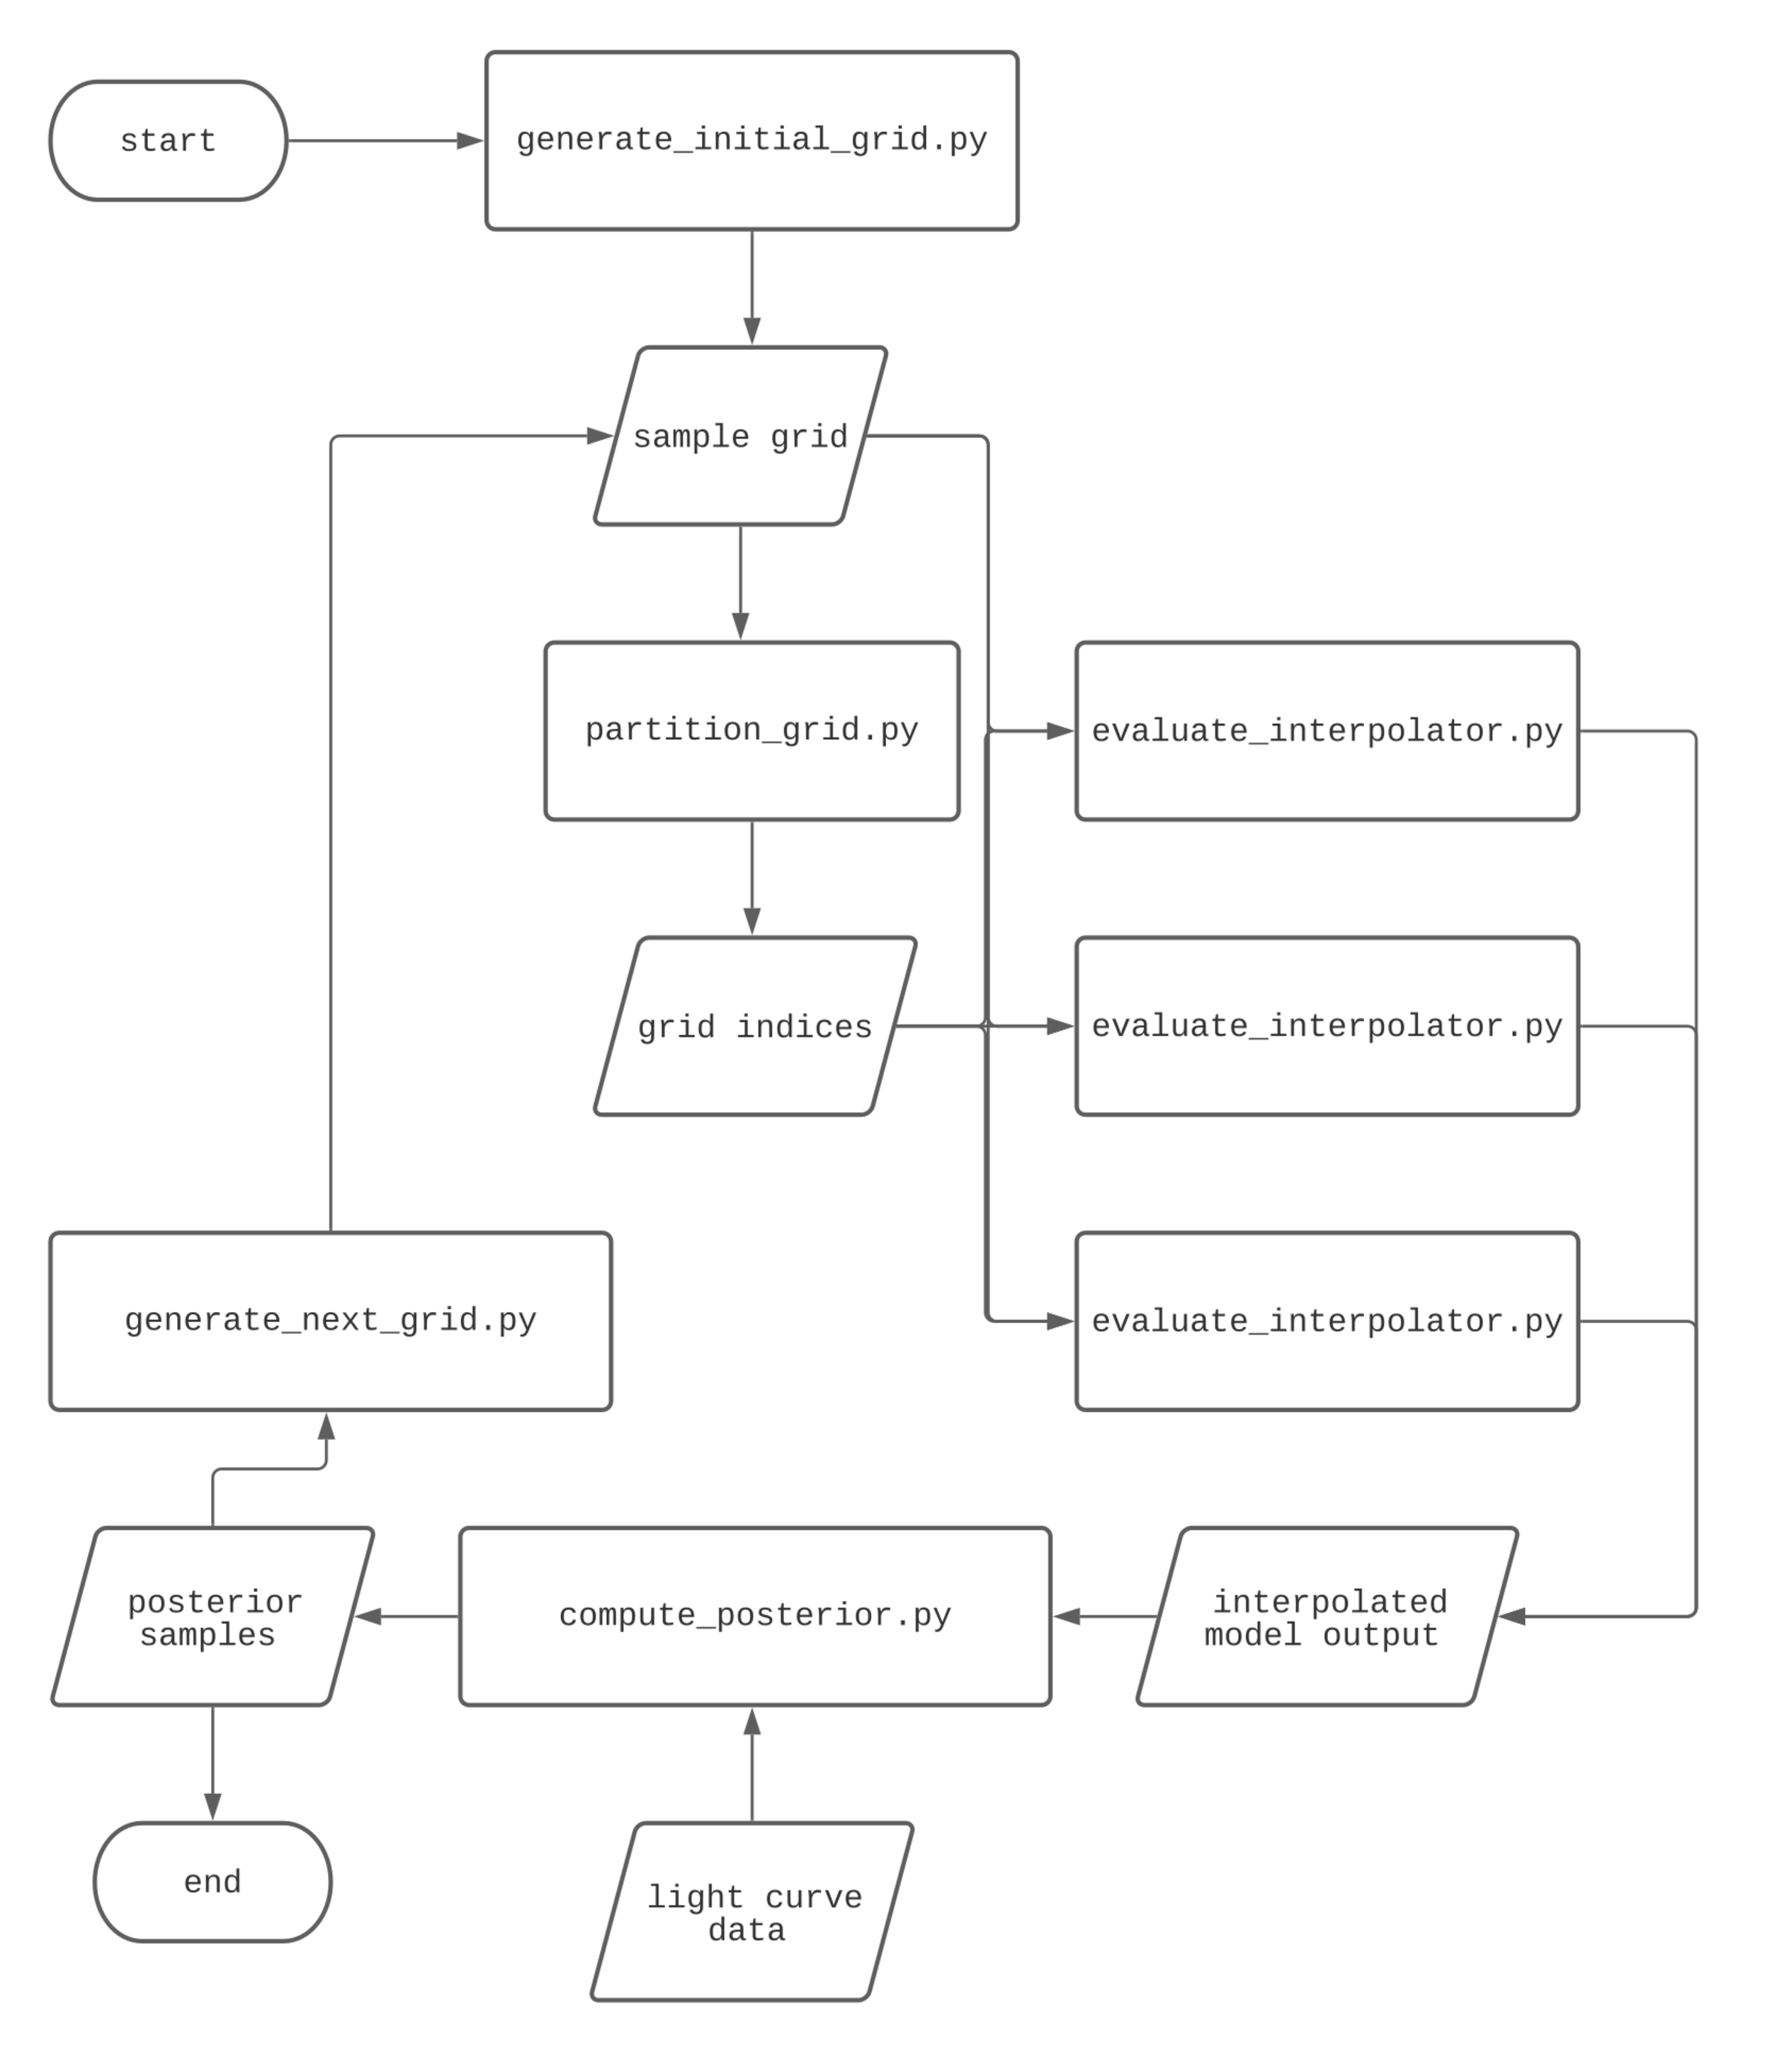
\includegraphics[width=\textwidth]{lc_fit_flowchart.pdf}	\caption{Flowchart depicting how data flows between individual scripts in the \texttt{lc\_fit} algorithm. Rectangles represent \texttt{Python} scripts, while parallelograms represent data. The \texttt{evaluate\_interpolator.py} block is only shown three times; however, in practice, many instances of this script run simultaneously}
	\label{fig:flowchart}
\end{figure}

\section{Interpolator evaluation}

The surrogate kilonova model consists of many Gaussian process (GP) interpolators that are saved elsewhere on the system; see \cite{ristic2021}. Each of these interpolators is trained at a specific viewing angle and post-merger time.

In order to best approximate the model at the times required by the observations, we evaluate the interpolators immediately before and after every observation in time. Because the observational data exists prior to setting up the PE run and does not change over the course of a PE run, the required interpolator times are known and can be used when generating the DAG.

Determining which of the fixed interpolator angles are needed is handled similarly: the angles immediately above and below each angle in the parameter grid are used. However, since the grid changes from one iteration to the next, there is no way to determine which angles are needed prior to runtime. The \texttt{partition\_grid.py} stage of the algorithm handles this by generating a list of grid indices corresponding to each fixed interpolator angle. The \texttt{evaluate\_interpolator.py} script takes interpolator time and interpolator angle as arguments, reads the corresponding grid indices from the files produced by \texttt{partition\_grid.py}, then evaluates the interpolator at the time and angle given to it for each grid point specified in the index file. Since all of these interpolator evaluations are independent, they are done in parallel.

In order to lighten the load on each individual interpolator job, the interpolated light curve values for every wavelength band are also computed as separate jobs. Each of these jobs saves its output (magnitudes and uncertainties in magnitude) to a file labeled by time, angle, and wavelength band. This information allows subsequent steps in the algorithm to reconstruct full light curves with uncertainties. In practice this step of the algorithm requires between 1,000 and 2,000 jobs, depending on the number of observations and other factors specific to a PE run. This highly parallel approach significantly decreases the time required for parameter estimation as compared to previous approaches. In principle this stage could be completed in a matter of minutes, limited only by the number of available nodes on a cluster.

\section{Computing the posterior samples}

Given a parameter vector $\bm{\theta}$ and a set of observations $\{x_i\}$, the posterior probability follows from Bayes' Theorem. Let $p(\bm{\theta})$ be the prior distribution and let and $\mathcal{L}(\{x_i\} \mid \bm{\theta})$ be the likelihood function, then the posterior probability is (up to proportionality)
\begin{equation} \label{eq:post}
	p (\bm{\theta} \mid \{x_i\}) \propto p(\bm{\theta}) \mathcal{L}(\{x_i\} \mid \bm{\theta}).
\end{equation}

The form of the likelihood function follows from the assumption of Gaussian noise:
\begin{equation} \label{eq:lnL}
	\mathcal{L}(\{x_i\} \mid \bm{\theta}) = \exp \left \{
			- \frac 1 2 \sum_i \left [ \frac {(m_i(\bm{\theta}) - x_i)^2}
			{\sigma_i^2 + \sigma_{i, \text{GP}}^2}
			+ \log \left (
				2 \pi \left ( 
					\sigma_i^2 + \sigma_{i, \text{GP}}^2
				\right )
			\right ) \right ]
	\right \},
\end{equation}
where $m_i(\bm{\theta})$ denotes the light curve model evaluated at the same time and in the same wavelength band as the observation $x_i$, $\sigma_i$ is the uncertainty in observation $x_i$, and $\sigma_{i, \text{GP}}$ is the uncertainty in the Gaussian process interpolation at $x_i$.

To calculate the likelihood, we must interpolate the Gaussian process outputs in both time and angle. The \texttt{compute\_posterior.py} script loads all of the Gaussian process outputs generated by \texttt{evaluate\_interpolator.py}, then using the index files produced by \texttt{partition\_grid.py}, reorders the interpolator outputs to match the original sample ordering in the grid. It then performs a linear interpolation in angle at each fixed interpolator time, followed by a linear interpolation in time to construct a full light curve, facilitating the likelihood calculation. The same procedure is followed for the Gaussian process uncertainties to obtain uncertainty as a function of time.

With the full light curves constructed, the likelihood calculation is straightforward. The likelihoods, priors, sampling priors (see Section \ref{sec:grid}), and samples are saved as the output of the algorithm.

\section{Grid generation} \label{sec:grid}

The initial sample grid is generated from the parameters' prior distributions. Subsequent grids, however, should ideally be sampled according to the posterior distribution itself. The process of adapting the sampling distribution so as to converge to the posterior is central to Bayesian parameter inference.

Suppose we have a grid sampled according to some sampling distribution $p_s(\bm{\theta})$. The posterior distribution, then, can be seen as a set of samples weighted by the ratio of the posterior probability (Eq. (\ref{eq:post})) to this sampling prior:
\begin{equation} \label{eq:weight}
	w(\bm{\theta}) \propto \frac {p(\bm{\theta} \mid \{x_i\})} {p_s(\bm{\theta})}.
\end{equation}
As the sampling distribution converges to the posterior distribution, these weights become essentially uniform. The \texttt{generate\_next\_grid.py} script samples a new parameter grid from an approximation of the posterior distribution, which is used in the next iteration of the algorithm.

The approximation scheme utilized in \texttt{lc\_fit} is a kernel density estimate (KDE) \editremark{[add a citation or two here]}. KDEs provide non-parametric estimates of probability distributions from which new samples can be drawn. The \texttt{scikit-learn} package provides a fast, simple KDE implementation that can be trained on weighted samples, and is therefore ideal for our purposes.

A common source of difficulty when using KDEs is choosing an appropriate value for the bandwidth, a hyperparameter describing the width of each (in our case, Gaussian) kernel. An appropriate value is chosen by \texttt{generate\_next\_grid.py} using the \texttt{scikit-learn} \texttt{GridSearchCV} object, which performs a cross-validation test to determine which value of a given hyperparameter leads to the best performance on a test set. In particular, 5-fold cross-validation is performed and the KDE with the highest ``score''--that is, log-probability of the test set under the model--is chosen.

Once an appropriate bandwidth has been found, a KDE is trained on the full sample set, then new samples are drawn from it. These samples are ``scored'' by the KDE, resulting in the sampling prior values $p_s(\bm{\theta})$. These samples and sampling prior values are saved as a new grid, which is used in the next iteration of the algorithm.

One potential problem with our approach, which is particularly important in early iterations, is the fact that when the sampling distribution is much more broad than the posterior distribution, a few points in the grid can have significantly higher weights than the rest. This causes problems when training the KDE, and can cause the algorithm to ``get stuck'' sampling the same point over and over. To alleviate this, a \texttt{--tempering-exponent} argument supplied to \texttt{generate\_next\_grid.py} is used. This argument is a number between 0 and 1 by which we multiply the log-likelihood (or, equivalently, exponentiate the likelihood). This has the effect of flattening and broadening the distribution on which the KDE is trained, preventing the aforementioned problems. This exponent typically begins at 0.001 or 0.01 in early iterations, and is gradually increased to 1, helping the algorithm to gradually converge to the posterior distribution. The starting value and number of iterations over over which it is increased are currently specified by the user, though this could be automated in the future. Note that because it is properly accounted for in the KDE, and therefore the sampling prior, this method does not bias our results.

\section{Setting up the DAG file}

At a high level, the \texttt{lc\_fit} algorithm requires the us to run many jobs in parallel, wait for them all to complete, run several scripts which each depend on the previous, then repeat. This process is automated using \texttt{HTCondor}, and the high-level structure of the algorithm is represented in the \texttt{HTCondor} DAG file (DAG stands for ``Directed Acyclic Graph'').

Each line of a DAG file generated by \texttt{lc\_fit} is one of four types:
\begin{enumerate}
	\item A \texttt{JOB} command, which instantiates a single \texttt{HTCondor} job by referring to a submit file.
	\item A \texttt{VARS} command, which specifies variable names and values to supply to the submit file for a given job, allowing a single submit file to be used for many different cases of the same computation.
	\item 	A \texttt{RETRY} command, specifying the number of times to retry a failed job.
	\item A \texttt{PARENT{\ldots}CHILD{\ldots}} command indicating that a given job (the \texttt{CHILD}) depends on another job (the \texttt{PARENT}) having been completed first.
\end{enumerate}

The DAG is automatically generated by the \texttt{dag\_setup.py} script. Given an input grid, \texttt{dag\_setup.py} adds an entry for the \texttt{partition\_grid.py} stage of the algorithm. Then, using the observational data, it determines which interpolators are needed to compute magnitudes at the required times, and creates a DAG entry for each one. Additional entries are then added for \texttt{compute\_posterior.py} and \texttt{generate\_next\_grid.py}, and the process is repeated for the number of iterations specified by the user.

\bibliographystyle{plain}
\bibliography{bibliography}

\end{document}
